\documentclass[12pt,english]{article}
\usepackage[english]{babel}
\usepackage{graphicx}
\usepackage{amsmath}
\usepackage{multirow}
\usepackage{pgfplots}
\usepackage{subcaption}
\usepackage{amssymb}
\usepackage[hidelinks]{hyperref}
\usepackage{caption}
\usepackage{amsthm}
\usepackage{multicol}
\pgfplotsset{compat=1.16}
\usepackage{minted}
\usepackage{float}
\usepackage{titling}
\usepackage{soul}
\usepackage{listings}
\newenvironment{statement}{\fontfamily{ptm}\selectfont}{\par}
\usepackage{array}
\graphicspath{ {../img/} {./img}}
\selectlanguage{english}
\usepackage[nottoc]{tocbibind}
\usepackage[utf8]{inputenc}
\usepackage{graphicx}
\usepackage[a4paper,left=2cm,right=2cm,top=2.5cm,bottom=2.5cm]{geometry}
\RecustomVerbatimEnvironment{Verbatim}{BVerbatim}{}


\title{Evolutionary Algorithms}
\setlength{\droptitle}{10em}
\author{Carlos Sánchez Páez}

\makeindex
\begin{document}


\begin{titlepage}

\newlength{\centeroffset}
\setlength{\centeroffset}{-0.5\oddsidemargin}
\addtolength{\centeroffset}{0.5\evensidemargin}
\thispagestyle{empty}

\noindent\hspace*{\centeroffset}
\begin{minipage}{\textwidth}

\centering

\includegraphics[width=0.75\textwidth]{bme_logo.jpg}\\[1.4cm]

\textsc{ \Large Evolutionary Algorithms\\[4cm]}

\textsc{\Huge Homework}\\[0.75cm]

{\Large\bfseries Ninth task\\}
\end{minipage}

\vspace{8cm}
\noindent\hspace*{\centeroffset}
\begin{minipage}{\textwidth}
\centering

\textbf{Author}\\ {Carlos Sánchez Páez}\\
\texttt{http://www.github.com/csp98}\\[0.5cm]
\textsc{Budapest University of Technology and Economics}\\
\vspace{1cm}
\textsc{Academic year 2018-2019}
\end{minipage}
\end{titlepage}
\thispagestyle{empty}

\newpage


\begin{enumerate}

	\item
		\begin{statement}
		Calculate the probability density function which is used to generate the new points in simulated annealing. With the help of the probability density function determine the expected value and standard deviation of the added random variable.
		\end{statement}


	\item
		\begin{statement}
		What might be the advantage of using global crossover compared to making offspring from two parents? Which leads to a higher convergence rate and why?
		\end{statement}
		By using global crossover it is possible to have different parents in each coordinate, so more variety is asured. Thanks to this, we can avoid getting stuck in a local maximum, so the convergence is faster.\\
		With two-parents offsprings we don't have such variety, so we can get stuck in a local maximum.
	\item
		\begin{statement}
			The Rosenbrock function is defined as:
			\begin{center}
				$f(x,y)=100(y-x^2)^2 + (x-1)^2$
			\end{center}
			Find every local and global extreme values by investigating the gradient. By examining the Hessian decide if it’s a long valley type function or not.
		\end{statement}
		I designed a program in Matlab to do this exercise. We can see that there is a local minimum placed at (1,1) and that it is strictly convex. This means that, in fact, it is a long valley type function.

		\item
			\begin{statement}
				 Implement Rechenberg’s algorithm for two variable functions. Your program has to plot the possible solutions and the function’s surface. Test your program with the Rosenbrock function, choosing the origin as starting point.
			\end{statement}
			By doing three iterations, this is the result of my program:
			\begin{figure}[H]
				\centering
				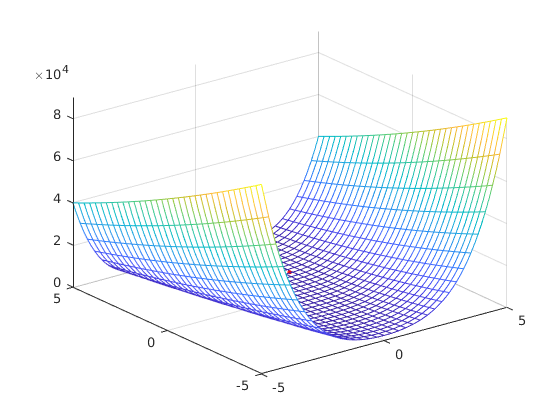
\includegraphics{ex4}
			\end{figure}

\end{enumerate}


\begin{thebibliography}{9}

\bibitem{Course Webpage}
Course Webpage
\\\texttt{http://math.bme.hu/~safaro/evolalgen.html}


\bibitem{Webpage4}
\texttt{https://tex.stackexchange.com/}


\end{thebibliography}


\end{document}
